% ycb1-fig-autonomic-nervous-system. Labels from notes block ycb1-hl-human-body-introduction
% ("Nervous" bullet and the deck layer: fight or flight, rest and digest; checked).
\documentclass[border=6pt]{standalone}
% Shared preamble for the YCB1 line diagrams (standalone TikZ, XeTeX). Black and white only; labels come from
% the checked notes block named in each diagram file. Build: make_figures.bat in this folder.
\usepackage{fontspec}
\setmainfont{Segoe UI}
\usepackage{tikz}
\usetikzlibrary{arrows.meta,positioning,shapes.geometric,calc,decorations.pathreplacing}
\hyphenpenalty=10000 \exhyphenpenalty=10000 % no hyphenated labels
\tikzset{
  box/.style={draw, rounded corners=2pt, align=center, inner sep=4pt, font=\small, minimum height=1.6em},
  head/.style={box, font=\small\bfseries},
  note/.style={align=center, font=\footnotesize},
  link/.style={-{Stealth[length=2mm]}, thin},
}

\begin{document}
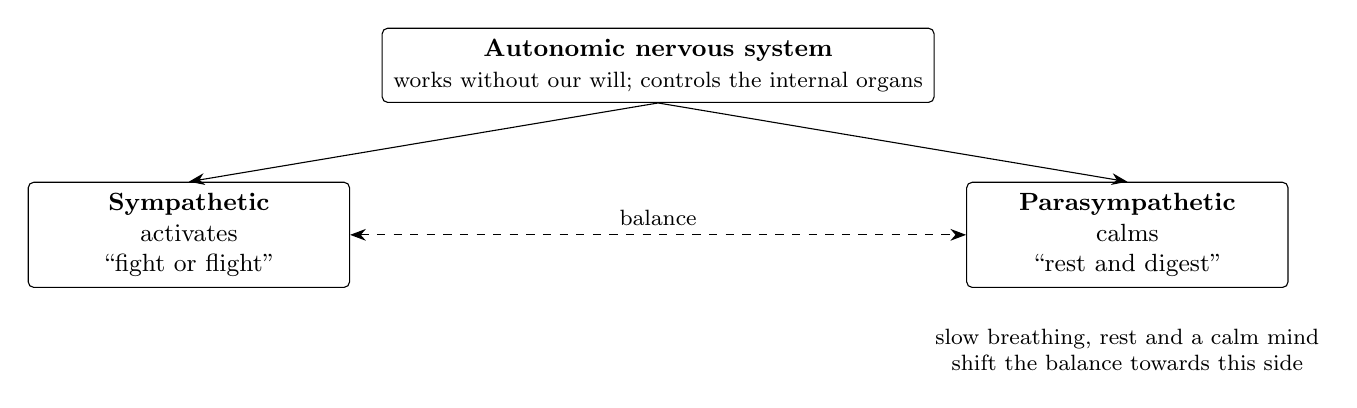
\begin{tikzpicture}
\node[head] (ans) {Autonomic nervous system\\{\normalfont\footnotesize works without our will; controls the internal organs}};
\node[box, below left=10mm and 4mm of ans, text width=38mm] (sym) {\textbf{Sympathetic}\\activates\\``fight or flight''};
\node[box, below right=10mm and 4mm of ans, text width=38mm] (par) {\textbf{Parasympathetic}\\calms\\``rest and digest''};
\draw[link] (ans.south) -- (sym.north);
\draw[link] (ans.south) -- (par.north);
\draw[{Stealth[length=2mm]}-{Stealth[length=2mm]}, dashed] (sym.east) -- node[above, note] {balance} (par.west);
\node[note, below=4mm of par] {slow breathing, rest and a calm mind\\shift the balance towards this side};
\end{tikzpicture}
\end{document}
